\chapter{Introdução}


O desenvolvimento de software usualmente enfrenta problemas relacionados ao não cumprimento dos prazos de entrega. Tal situação pode ocorrer devido ao aumento de demandas não planejadas no início do projeto, desvios na interpretação e/ou implementação dos requisitos, bem como problemas internos na equipe. Assim, a solução para atrasos de entrega pode estar em soluções que resolvam problemas específicos. Vale ressaltar que a literatura apresenta estratégias que podem mitigar ou combater esse problema, como por exemplo, o reuso de software. Este trabalho de conclusão de curso propõe uma solução de padronização do controle de acesso dos softwares, abstraindo-o e tornando-o passível de maior reuso como um serviço reutilizável no desenvolvimento de software, reduzindo assim o tempo de desenvolvimento e manutenção de aplicações de software. O capítulo corrente é composto por sete seções. A Seção \ref{motivacao} aborda a motivação do trabalho, a Seção \ref{problema} o problema do contexto, a Seção \ref{objetivos} mostra os objetivos almejados, a Seção \ref{metodologia} comenta sobre a metodologia aplicada, a Seção \ref{resultados} demonstra os resultados esperados com a aplicabilidade do trabalho proposto, a Seção \ref{fora} discorre sobre elementos fora do escopo do projeto e por fim, a Seção \ref{estrutura} exibe a estrutura da monografia.


\section{Motivação}\label{motivacao}


Otimizar o desenvolvimento de software é uma tarefa bastante estudada, com uma vasta literatura. A área de Engenharia de Software estuda maneiras de melhorar o desenvolvimento de software mediante processos e práticas de desenvolvimento. Qualquer melhoria durante a construção de um sistema, normalmente acaba por prover uma economia no orçamento de desenvolvimento e/ou manutenção, bem como a redução no tempo de entrega dos projetos. Assim, é possível que melhorias no processo de desenvolvimento de sistemas, podem satisfazer desde as necessidades do programador, com um trabalho facilitado, até às necessidades do cliente final, com a redução de custo.


\section{Problema}\label{problema} %começar de forma mais genérica

A reutilização não-sistemática de trechos de código é um problema que pode acarretar no aumento da complexidade do software, bem como no tempo de desenvolvimento e manutenção. Este problema atinge fortemente a manutenibilidade do software, o que pode gerar grande transtorno diante de uma alteração que poderia ser simples caso o projeto fosse concebido considerando o potencial de reuso. Deste modo, a reutilização sistemática de código é uma prática bem-vinda em projetos de software. A abordagem de reuso pode inclusive, abranger mais de um projeto numa organização, possibilitando que módulos inteiros sejam reaproveitados. 


\section{Objetivos}\label{objetivos}


\begin{itemize}
	\item \textbf{Objetivo geral}: O objetivo geral do ModMan é prover o reuso de código, utilizando padões que mantenham o componente de código na melhor forma possível para ser acoplado em outros softwares de modo facilitado.
	\item \textbf{Objetivo específico}: Neste trabalho, buscamos implementar um mecanismo de reutilização de módulo de controle de acesso de um sistema, já que o mesmo está presente sem remodelações nos sistemas de uma organização. Assim, o objetivo foi desenvolver tal módulo como um serviço, deixando-o isolado e gerando a possibilidade de qualquer sistema consumir tal módulo como um serviço. Dessa forma, ao projetar um novo software para uma organização por exemplo, ao invés de incluir o módulo de controle de acesso, projetaria-se o código para consumir o serviço de controle de acesso, o qual seria um projeto à parte. Também apresenta a vantagem de ter interoperabilidade entre linguagens de programação, já que realiza a comunicação através de JSON (JavaScript Object Notation), seguindo padrões atuais. Assim, tem-se uma constância no módulo de acesso independentemente da possível necessidade de migração de tecnologia.
\end{itemize}


\section{Metodologia}\label{metodologia}
%<como será feito, como resolver o problema apontado inicialmente>
Esta seção apresenta as tecnologias utilizadas na implementação do ModMan com base na indústria de desenvolvimento de software (estado da prática). Para embasar esse cenário, a seguir apresentamos dados que refletem a atual situação do mercado, a nível global.


%INSERIR AQUI FALANDO DA METODOLOGIA, ARQUITETURA, QUE SAO USADOS...


%<analise de literatura | design | implementação | validação>
Baseando-se nas tecnologias livres comummente empregadas no cenário atual do desenvolvimento Web, há diversas opções eficientes para a implementação da solução. Dentre as possibilidades, considerando a facilidade para futura manutenção e continuidade do projeto, tende-se a optar por uma tecnologia popular. Como linguagem de programação, a proposta deste trabalho foi desenvolvida utilizando o PHP (PHP: Hypertext Preprocessor). A escolha é fundamentada na pesquisa da RedMonk de 2015 \cite{Grafico-RedMonk}, que evidencia o uso das linguagens de programação de acordo com as discussões no StackOverflow\footnote{http://pt.stackoverflow.com/} e repositórios no GitHub\footnote{github.com}. A Figura \ref{fig:graficoRedmonk} apresenta a popularidade das liguagens de programação, na qual o PHP é apresentado na terceira colocação, apenas atrás do líder, JavaScript, e do segundo colocado, Java.


\begin{figure}
	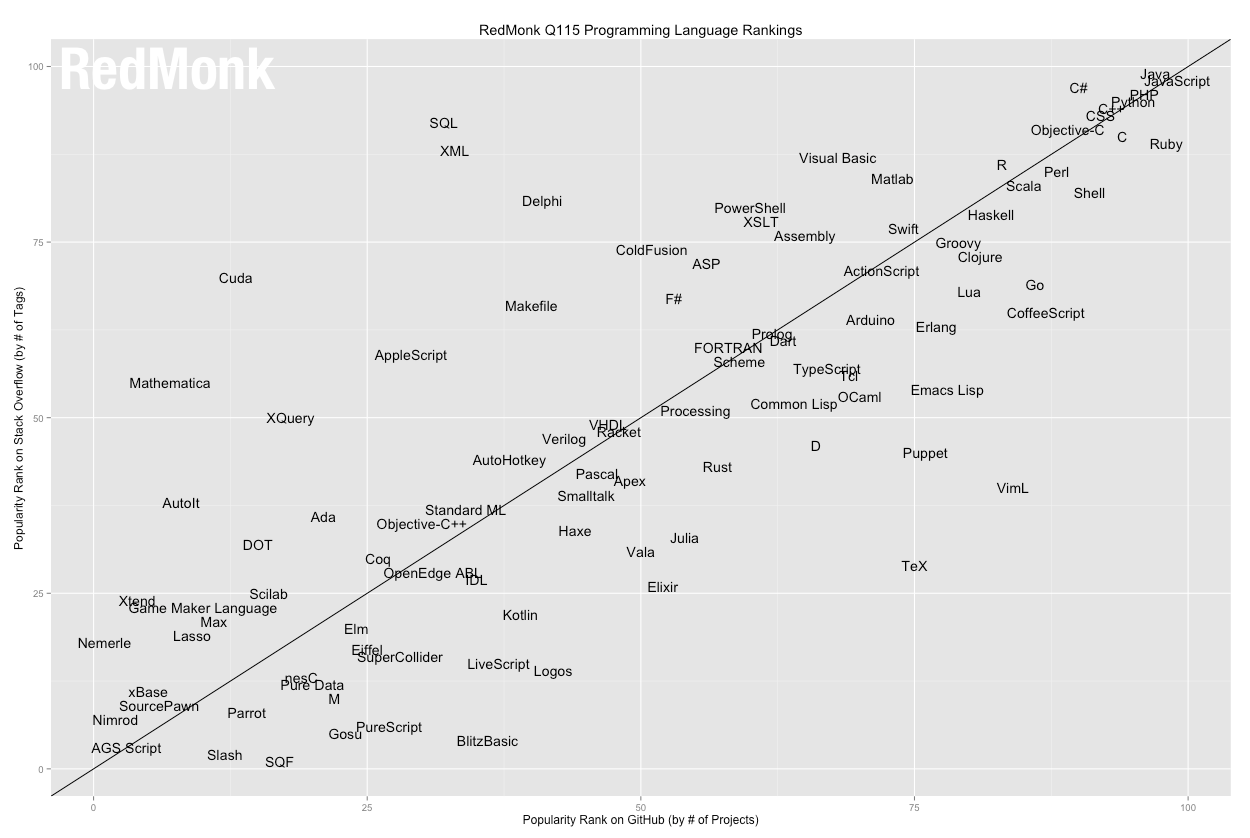
\includegraphics[width=1\textwidth]{images/grafico_redmonk}
	\caption{Ranking das liguagens de programação no Stack Overflow e Github}
    \label{fig:graficoRedmonk}
\end{figure}


Adicionalmente, dentre os frameworks disponíveis para PHP, de acordo com a Figura \ref{fig:graficoWebhostface}, hoje o destaque está com o Laravel\footnote{https://laravel.com/}, que se encontra como o mais utilizado no momento.
 

A WebHostFace\footnote{https://www.webhostface.com/}, uma empresa de hospedagem, compilou várias estatísticas para criar um infográfico mostrando os frameworks PHP mais populares de 2015. Utilizando informações sobre os próprios clientes, o Google Trends, estatísticas de repositórios do GitHub e a pesquisa do SitePoint “Best PHP Frameworks 2015”, a WebHostFace elaborou o infográfico apresentado na figura \ref{fig:graficoWebhostface}.


\begin{figure}
	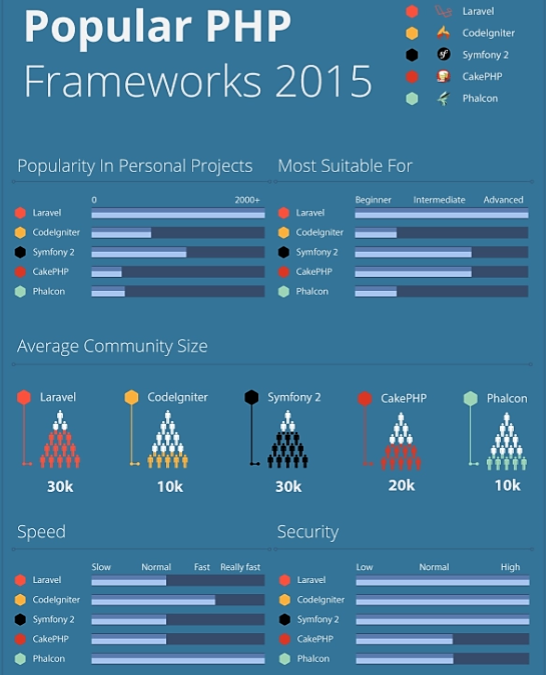
\includegraphics[width=1\textwidth]{images/infografico_webhostface}
	\caption{Infográfico da WebhostFace, exibindo a popularidade dos Frameworks PHP em 2015}
    \label{fig:graficoWebhostface}
\end{figure}


De acordo com a Figura \ref{fig:graficoWebhostface}, o Laravel em 2015 teve a maior popularidade em projetos pessoais e tem a maior comunidade entre os concorrentes. Além disso, em comparação aos concorrentes, tem alto nível de segurança e velocidade de resposta com nível normal. Tais características analisadas na Figura \ref{fig:graficoRedmonk}, tornam o Laravel uma boa escolha para a escrita de um software que possivelmente será mantido por terceiros.


Para elaborar os recursos de interface e integrar ao back-end PHP do sistema, será adotado o AngularJS\footnote{https://angularjs.org/}, ferramenta sólida e conhecida no aspecto em questão. 


Dados coletados via Google Trends, que propõem comparações entre termos pesquisados, revelam a popularidade do AngularJS diante de alguns dos principais concorrentes. O gráfico \ref{fig:graficoGoogleTrendsFerramentasFront} evidencia o cenário, mostrando que o AngularJs lidera como termo pesquisado dentre framwworks relacionados.


\begin{figure} % \ref{fig:graficoGoogleTrendsFerramentasFront}. 
	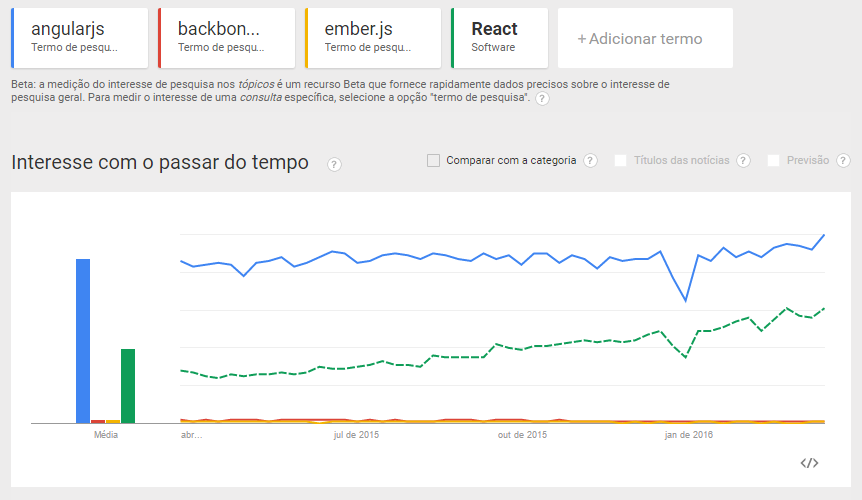
\includegraphics[width=1\textwidth]{images/grafico_ferramentas_front}
	\caption{Gráfico do Google Trends exibindo as pesquisas por ferramentas front-end}
    \label{fig:graficoGoogleTrendsFerramentasFront}
\end{figure}


\section{Resultados Esperados}\label{resultados}


A partir do uso do proposto módulo de controle de acesso como serviço, espera-se que ocorram os seguintes ganhos:


\begin{itemize}
	\item Servir a projetos de diferentes linguagens;
	\item Atender a projetos de diferentes plataformas (Web, Desktop, Mobile);
	\item Facilitar a configuração das permissões;
	\item Extinguir o módulo de permissões nos projetos em que o trabalho proposto será aplicado.
\end{itemize}


\section{Fora de Escopo}\label{fora}


As permissões de acesso podem estar disponíveis mediante diversas configurações. Por exemplo, pode ser condicional ao pagamento da mensalidade. Essas características que tendem a levar o ModMan para se assemelhar a um ERP (Enterprise Resource Planning), não estão no escopo da implementação apesar de ser possível que o ModMan adquira essas caracterísitcas mediante evoluções no sistema. Atualmente, o ModMan é um sistema limitado, que restringe a sua atuação somente às permissões de acesso numa forma simples.
%Diante da possibilidade de gerência dos sistemas, módulos e funcionalidades contratadas, seria possível estender o ModMan, complementando-o com uma abordagem financeira, controlando o acesso do cliente mediante o pagamento do que está contratado pelo cliente. Também existe a possibilidade de realizar o controle por número de usuários que estão logados no sistema contratado ou por módulo, mediante uma evolução na implementação. Uma possível solução para a última situação seria o sistema consumidor enviar uma notificação (post) ao sistema de gerenciamento de módulo num determinado intervalo de tempo, sinalizando o usuário logado no sistema. O sistema de gerenciamento de módulos/permissões responderia internamente à sinalização, mantendo registro de usuário ativo. Caso o usuário final saia do sistema, enviaria o sinal de logout e caso fechasse o navegador, a sessão seria encerrada por tempo de inatividade (falta de envio da notificação de uso).


\section{Estrutura do Trabalho}\label{estrutura} %<breve resumo sobre os capítulos do TCC>


Nesta seção, tem-se uma breve apresentação dos demais capítulos que compõem este trabalho de conclusão de curso:

\begin{itemize}
    \item Capítulo 2: \textit{Referencial teórico}, fundamentando os principais conceitos que compõem os elementos principais do trabalho;
	\item Capítulo 3: \textit{Proposta}, contendo o detalhamento do trabalho proposto, baseando-se nos aterfatos da engenharia de software;
	\item Capítulo 4: \textit{Avaliação empírica}, apresentando a prova de conceito do trabalho;
	\item Capítulo 5: \textit{Conclusão}, apresentando o desfecho do trabalho.
\end{itemize}

